\tikzset{>=latex} % for LaTeX arrow head
\contourlength{1.4pt}

\colorlet{Ecol}{orange!90!black}
\colorlet{EcolFL}{orange!90!black}
\colorlet{veccol}{green!45!black}
\colorlet{EFcol}{red!60!black}
\tikzstyle{charged}=[top color=blue!20,bottom color=blue!40,shading angle=10]
\tikzstyle{darkcharged}=[very thin,top color=blue!60,bottom color=blue!80,shading angle=10]
\tikzstyle{charge+}=[very thin,top color=red!80,bottom color=red!80!black,shading angle=-5]
\tikzstyle{charge-}=[very thin,top color=blue!50,bottom color=blue!70!white!90!black,shading angle=10]
\tikzstyle{darkcharged}=[very thin,top color=blue!60,bottom color=blue!80,shading angle=10]
\tikzstyle{gauss surf}=[green!70!black,top color=green!2,bottom color=green!80!black!70,shading angle=5,fill opacity=0.6]
\tikzstyle{gauss lid}=[gauss surf,middle color=green!80!black!20,shading angle=40,fill opacity=0.7]
\tikzstyle{gauss dark}=[green!60!black,fill=green!60!black!70,fill opacity=0.8]
\tikzstyle{gauss line}=[green!80!black]
\tikzstyle{gauss dashed line}=[green!60!black!80,dashed,line width=0.2]
\tikzstyle{vector}=[->,thick,veccol]
\tikzstyle{normalvec}=[->,thick,blue!80!black!80]
\tikzstyle{EField}=[->,thick,Ecol]
\tikzstyle{EField dashed}=[dashed,Ecol,line width=0.6]
\tikzset{
  EFieldLine/.style={thick,EcolFL,decoration={markings,
                     mark=at position #1 with {\arrow{latex}}},
                     postaction={decorate}},
  EFieldLine/.default=0.5}
\tikzstyle{measure}=[fill=white,midway,outer sep=2]
\def\L{2.2}
\def\H{2.2}
\def\offset{2.0}
\def\W{0.30}
\def\Nx{5}
\def\Ny{5}

% PLANE charge distribution





% PLANE field with gaussian surface


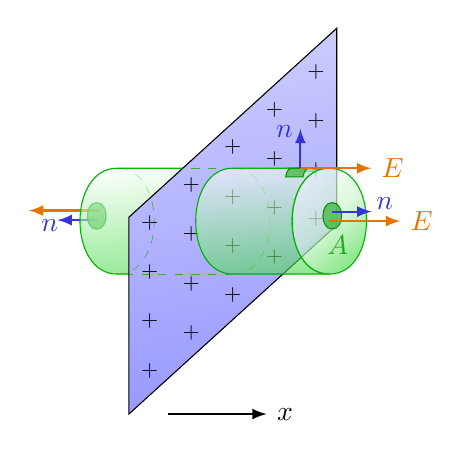
\begin{tikzpicture}[x={(1.0cm,0)},y={(0.55cm,0.5cm)},z={(0,1.0cm)}]
  \def\H{2.5}
  \def\W{4.8}
  \def\Ny{5}
  \def\Nz{4}
  \def\R{0.14*\W}
  \def\a{0.49*\H}
  \def\E{0.36*\H}
  \def\plane{(0,0,0) --++ (0,\W,0) --++ (0,0,\H) --++ (0,-\W,0) -- cycle;}
  \coordinate (O) at (0.0,-0.5,-0.5);
  \coordinate (C)  at (      0,\W/2,\H/2);
  \coordinate (ER) at (     \a,\W/2,\H/2);
  \coordinate (EL) at (-1.2*\a,\W/2-0.6*\R,\H/2+0.5*\R);
  \coordinate (TM) at (      0,\W/2,\H/2+\R);
  \coordinate (TR) at (     \a,\W/2,\H/2+\R);
  \coordinate (TL) at (-1.2*\a,\W/2,\H/2+\R);
  \coordinate (BM) at (      0,\W/2,\H/2-\R);
  \coordinate (BR) at (     \a,\W/2,\H/2-\R);
  \coordinate (BL) at (-1.2*\a,\W/2,\H/2-\R);
  \coordinate (NT) at (0.7*\a,\W/2,\H/2+\R);
  \coordinate (NR) at (\a,\W/2+0.13*\R,\H/2+0.13*\R);
  \coordinate (NL) at (-1.2*\a,\W/2-0.5*\R,\H/2-0.2*\R);
  \coordinate (NB) at (0.86*\a,\W/2-0.6*\R,\H/2-0.6*\R);
  
  % AXES
  \draw[->,thick] (0.5,0,0) --++ (0.5*\H,0,0) node[right] {$x$};
  
  % VECTORS back
  \draw[EField] (EL) --++ (-\E,0,0);
  \draw[normalvec] (EL) ++(0,-0.1*\R,-0.13*\R) --++ (-0.5,0,0) node[below left=-4] {$\vu{n}$};
  \draw[gauss dark]
    (EL)++(0,-0.1*\R,-0.3*\R)
      to[out=0,in=0,looseness=1.2] ++(0,0,0.5*\R)
      to[out=180,in=180,looseness=1.2] ++(0,0,-0.5*\R) -- cycle; %node[left=4,below=-1] {$\dd{A}$};
  
  % GAUSSIAN SURFACE back
  \draw[gauss dashed line] (BL) to[out=0,in=0,looseness=1.2] (TL);
  \draw[gauss surf]
    (BM) to[out=180,in=180,looseness=1.2] (TM) --
    (TL) to[out=180,in=180,looseness=1.2] (BL) -- cycle;
  
  % PLANE
  \draw[charged] \plane;
  \begin{scope}
    \clip \plane;
    \draw[gauss dashed line] (BM) -- (BL);
    \draw[gauss dashed line] (TM) -- (TL);
    \draw[gauss dashed line] (BL) to[out=0,in=0,looseness=1.2] (TL);
  \end{scope}
  \foreach \i [evaluate={\y=(\i-0.5)*\W/\Ny;}] in {1,...,\Ny}{
    \foreach \j [evaluate={\z=(\j-0.5)*\H/\Nz;}] in {1,...,\Nz}{
      \node[scale=0.8,rotate=0] at (0,\y,\z) {$+$};
    }
  }
  \draw[gauss dark]
    (NT) ++ (-0.12,0,0) to[out=-5,in=110] ++(0,0.12,-0.10) --++(0.22,0,0) to[out=110,in=-5] ++(0,-0.12,0.10) -- cycle;
  
  % GAUSSIAN SURFACE front
  \draw[gauss dashed line]
    (BM) to[out=0,in=0,looseness=1.2] (TM);
  \draw[gauss surf]
    (BM) to[out=180,in=180,looseness=1.2] (TM) --
    (TR) to[out=180,in=180,looseness=1.2] (BR) -- cycle;
  \draw[gauss lid]
    (BR) to[out=0,in=0,looseness=1.2] (TR) to[out=180,in=180,looseness=1.2] cycle;
  
  % DARK
  \draw[gauss dark]
    (NT) ++ (-0.12,0,0) to[out=-160,in=80] ++(0,-0.12,-0.05) --++(0.22,0,0) to[out=80,in=-160] ++(0,0.12,0.05) -- cycle;
  \draw[gauss dark]
    (ER)++(0,0.1*\R,-0.2*\R)
      to[out=0,in=0,looseness=1.2] ++(0,0,0.5*\R)
      to[out=180,in=180,looseness=1.2] ++(0,0,-0.5*\R) -- cycle node[right=2,below=-1] {$\dd{A}$};
  
  % ELECTRIC FIELD
  \draw[EField] (ER) --++ (\E,0,0) node[right] {$\vb{E}$};
  \draw[EField] (NT) --++ (\E,0,0) node[right] {$\vb{E}$};
  
  % VECTORS
  \draw[normalvec] (ER) ++(0,0.1*\R,0.13*\R) --++ (0.5,0,0) node[above=3,right=-2] {$\vu{n}$};
  \draw[normalvec] (NT) --++ (0,0,0.5) node[below=1,left=-1] {$\vu{n}$};
  %\draw[normalvec] (NB) --++ (0,-0.35,-0.25) node[below right=-2] {$\vu{n}$};
  
  
\end{tikzpicture}
